\setcounter{secnumdepth}{4}

\subsection{CheXNet}
In this project, led by Stanford ML Group, an algorithm was developed to interpret chest X-ray images and detect if Pneumonia is present while showing a heat map of the area in the image that had the highest activations \cite{rajpurkar2017chexnet}. Example output can be see in figure~\ref{fig:CheXNetExample}


\begin{figure}[H]
	\centering
	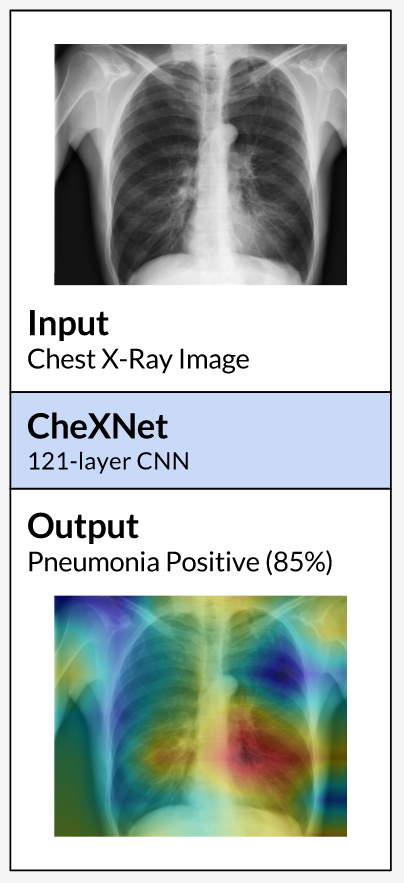
\includegraphics[scale=0.5]{HeatMap.png}
	\caption{Example of CheXNet output of class label along with probability from softmax layer and heat-map}
	\label{fig:CheXNetExample}
\end{figure}

Results showed that the algorithm can detect the pathology at a level exceeding radiologists. The algorithm used a 121-layer CNN which was trained on ChestX-ray14 \cite{wang2017chestx} which is currently the largest publicly available chest X-ray dataset, containing over 100,000 frontal view images and 14 different pathologies. The CNN used is based on the DenseNet architecture \cite{huang2017densely} but modifications were made for single output in the fully connected layer by applying a non-linearity sigmoid function, so that only Pneumonia would have a probability. Pre-trained weights were initialised from a model trained on ImageNet \cite{deng2009imagenet} to speed up the process of training. 
\subsubsection{Results}
Precautions were put in place to make sure that patient images between training and testing sets never overlap. In order to test the accuracy of the model, 420 chest X-rays were collected and 4 practising radiologists annotated where they think the Pneumonia is present. Through the CheXNet tests it showed the algorithm exceeds average radiologist performance on the \textbf{F1 metric}. The model was comparative with expert radiologists on metrics such as \textbf{accuracy}, \textbf{sensitivity} and \textbf{specificity}. The biggest difference was in terms of speed as radiologists took around 4 hours on average to interpret the images whereas CheXNet algorithm took less than 2 minutes \cite{rajpurkar2017chexnet}. Results from figure~\ref{fig:F1Score} present the F1 score for algorithm and average of the 4 clinicians. 

\begin{figure}[H]
	\centering
	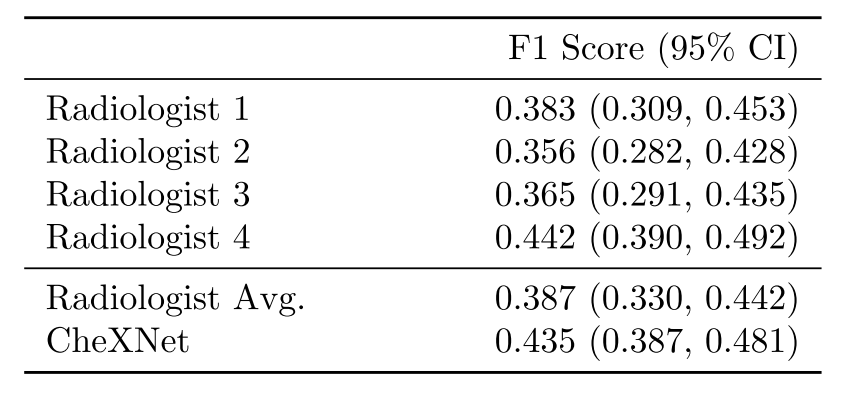
\includegraphics[scale=0.5]{F1Score.png}
	\caption{F1 Score for CheXNet and average F1 score for 4 radiologists}
	\label{fig:F1Score}
\end{figure}